\documentclass[aspectratio=169]{beamer}
\usepackage{amsmath}
\usepackage{amssymb}
\usepackage{minted}
\usepackage{graphicx}
\title{EM algorithm}
\subtitle{Maximum Likelihood Estimation of the t-distribution}
\author{Lucas Støjko Andersen}
\setminted{fontsize=\fontsize{8pt}{8pt}}
\institute{University of Copenhagen}
\date{\today}

\begin{document}
\begin{frame}
    \titlepage
\end{frame}
\begin{frame} x
    \frametitle{The t-distribution}
    \framesubtitle{The density of the non-standard t-distribution}
    The density of the t-distribution is given by
    \begin{equation}
        \label{eq:marginal}
        g(x)=\frac{\Gamma\left(\frac{\nu + 1}{2}\right)}{\sqrt{\pi\nu\sigma^2}\Gamma\left(\frac{\nu}{2}\right)}\left(1+\frac{(x - \mu)^2}{\nu\sigma^2}\right)^{-\frac{\nu + 1}{2}}
    \end{equation}
    with parameters $\mu\in\mathbf{R}$, $\nu > 0$, $\sigma^2 > 0$. Here, $\Gamma$ is the gamma function.\\[12pt]
    For independent observations $X_{1},X_{2},\ldots,X_{n}$ with density as in (\ref{eq:marginal}) there exist no nice analytic solutions to the MLE --- even with $\nu$ known.
\end{frame}
\begin{frame}
    \frametitle{There is another way}
    \framesubtitle{A joint approach with latent variables}
    Consider $(X, W)$ with density
    \begin{equation}
        \label{eq:join}
        f(x,w)=\frac{1}{\sqrt{\pi\nu\sigma^2}2^{(\nu+1)/2}\Gamma(\nu/2)}w^{\frac{\nu - 1}{2}}e^{-\frac{w}{2}\left(1+\frac{(x -\mu)^2}{\nu\sigma^2}\right)}
    \end{equation}
    Notice that $W\mid X = x \sim \Gamma(\alpha, \beta)$ --- the gamma distribution --- with parameters
    \begin{equation}
        \alpha = \frac{\nu + 1}{2} \quad\quad 
        \beta = \frac{1}{2}\left(1+\frac{(x -\mu)^2}{\nu\sigma^2}\right).
    \end{equation}
    This can be used to show that $X$ indeed has the marginal density of the t-distribution with parameters $\mu,\sigma^2,\nu$.
\end{frame}
\begin{frame}
    \frametitle{The Full Maximum Likelihood Estimate}
    \framesubtitle{MLE with fixed $\nu$}
    Assume $\nu>0$ known. I.i.d. $(X_{1},W_{1}), (X_{2},W_{2}),\ldots,(X_{n},W_{n})$ have log-likelihood
    \begin{equation}
        \ell(\theta)\simeq -\frac{n}{2}\log\sigma^2 -\frac{1}{2\nu\sigma^2}\sum_{i=1}^{n}W_{i}(X_{i}-\mu)^{2}.
    \end{equation}
    The solution is that of the weighted least squares:
    \begin{equation}
        \hat\mu =\frac{\sum_{i=1}^{n}W_{i}X_{i}}{\sum_{i=1}^{n}W_{i}},\quad\quad \hat\sigma^2 = \frac{1}{n\nu}\sum_{i=1}^{n}W_{i}(X_{i}-\hat\mu)^{2}.
    \end{equation}
\end{frame}
\begin{frame}[fragile]
    \frametitle{The Full Maximum Likelihood Estimate}
    \framesubtitle{MLE with fixed $\nu$ --- implemented in R}
    We can sample $(X,W)$ by sampling $W$ from a $\chi^{2}_{\nu}$ distribution and then sampling $X$ from a $\mathcal{N}(\mu, \nu\sigma^2/W)$.

\begin{minted}{R}
simulate_X <- function(N, mu, sigma, nu) {
    W <- rchisq(N, nu)
    X <- rnorm(N, mu, sqrt(nu * sigma / W))
    
    list(x = X, w = W)
}
    
full_mle <- function(X, W, nu) {
    mu <- sum(X * W) / sum(W)
    sigma <- sum(W * (X - mu)^2) / (nu * (length(X)))
    list(mu = mu, sigma = sigma)
}

set.seed(3939392)
samples <- simulate_X(100000, 5, 1.5, 3)
full_mle(samples$x, samples$w, 3)
\end{minted}
We obtain the estimates $\hat\mu_{\text{full}} = 4.997852$ and $\hat\sigma^{2}_{\text{full}}=1.500886$.
\end{frame}
\begin{frame}
    \frametitle{EM algorithm}
    \framesubtitle{MLE of the marginal likelihood for fixed $\nu$}
    Only $X$ is observed and so the full MLE cannot be computed. Using the EM algorithm we iteratively maximize the quantity
    \begin{equation}
        Q(\theta\mid\theta')=E_{\theta'}(\log f_{\theta}(X, W)\mid X)
    \end{equation}
    where $\theta = (\mu,\sigma^2)$. Using the log-likelihood from earlier
    \begin{equation}
        Q(\theta\mid\theta')\simeq -\frac{n}{2}\log\sigma^{2}-\frac{1}{2\nu\sigma^{2}}\sum_{i=1}^{n}E_{\theta'}(W_{i}\mid X_{i})(X_{i}-\mu)^{2}.
    \end{equation}
    The maximizer is then
    \begin{equation*}
        \hat\mu_{\theta'} =\frac{\sum_{i=1}^{n}E_{\theta'}(W_{i}\mid X_{i})X_{i}}{\sum_{i=1}^{n}E_{\theta'}(W_{i}\mid X_{i})},\quad \hat\sigma^{2}_{\theta'}= \frac{1}{n\nu}\sum_{i=1}^{n}E_{\theta'}(W_{i}\mid X_{i})(X_{i}-\hat\mu)^{2}.
    \end{equation*}
\end{frame}
\begin{frame}
    \frametitle{EM algorithm}
    \framesubtitle{E-step and M-step}
    The E-step boils down to computing $E_{\theta'}(W_{i} \mid X_{i})$
    \begin{equation}
        E_{\theta'}(W_{i} \mid X_{i}) = \frac{\alpha}{\beta}=\frac{\nu' + 1}{2}\frac{1}{\frac{1}{2}\left(1 + \frac{(X_{i} - \mu')^{2}}{\nu'\sigma'^{2}}\right)}=\frac{\nu' + 1}{1 + \frac{(X_{i}- \mu')^{2}}{\nu'\sigma'^{2}}}
    \end{equation}
    and doing the M-step by computing
    \begin{equation*}
        \hat\mu_{\theta'} =\frac{\sum_{i=1}^{n}E_{\theta'}(W_{i}\mid X_{i})X_{i}}{\sum_{i=1}^{n}E_{\theta'}(W_{i}\mid X_{i})},\quad \hat\sigma^{2}_{\theta'}= \frac{1}{n\nu}\sum_{i=1}^{n}E_{\theta'}(W_{i}\mid X_{i})(X_{i}-\hat\mu)^{2}.
    \end{equation*}
\end{frame}
\begin{frame}[fragile]
    \frametitle{EM algorithm}
    \framesubtitle{Implementation of marginal MLE}

\begin{minted}{R}
E_step <- function(x, nu) {
    #force(x)
    #force(nu)
    function(par) {
        # mu = par[1]
        # sigma^2 = par[2]
        (nu + 1) / (1 + ((x - par[1])^2) / (nu * par[2]))
    }
}

M_step <- function(x, nu) {
  #force(x)
  #force(nu)
  function(EW) {
    mu <- sum(EW * x) / sum(EW)
    sigma <- mean(EW * (x - mu)^2) / nu
    c(mu, sigma)
  }
}
\end{minted}

\end{frame}
\begin{frame}[fragile]
    \frametitle{EM algorithm}
    \framesubtitle{Implementation of marginal MLE}

\begin{minted}{R}
EM <- function(par, x, nu, maxit = 500, min.eps = 1e-7) {
    E <- E_step(x, nu)
    M <- M_step(x, nu)
    for(i in 1:maxit) {
        EW <- E(par)
        new_par <- M(EW)
        if(sum((new_par - par)^2) < min.eps * (sum(par^2) + min.eps)) {
            par <- new_par
            break
        }
        par <- new_par
        if(i == maxit) warning("Maximum number of itertaions reached.")
    }
    names(par) <- c("mu", "sigma")
    list(par = c(par, nu = nu), iterations = i)
}
\end{minted}

\end{frame}

\begin{frame}
    \frametitle{EM algorithm}
    \framesubtitle{Comparison of marginal MLE and full MLE}
    For starting values $\theta' = (1, 2)$ we obtain the estimates
    \begin{equation}
        \hat\mu_{\text{EM}}=4.995958,\quad\quad \hat\sigma^{2}_{\text{EM}}=1.504293,\quad\quad \nu = 3.
    \end{equation}
    in 9 iterations of the EM algorithm. Recall the full MLE
    \begin{equation}
        \hat\mu_{\text{full}} = 4.997852, \quad\quad \hat\sigma^{2}_{\text{full}}=1.500886,\quad\quad \nu = 3.
    \end{equation}
\end{frame}

\begin{frame}
    \frametitle{Robustness of the initial parameters}
    \framesubtitle{Properties of the t-distribution}
    The t-distribution has first moment if $\nu > 1$ and second moment if $\nu > 2$. When the moments exist then
    \begin{equation}
        EX = \mu,\quad\quad VX = \sigma^{2}\frac{\nu}{\nu + 2}.
    \end{equation}
    The calculations in the E-step may be unstable
    \begin{equation*}
        \hat\mu_{\theta'} =\frac{\frac{1}{n}\sum_{i=1}^{n}E_{\theta'}(W_{i}\mid X_{i})X_{i}}{\frac{1}{n}\sum_{i=1}^{n}E_{\theta'}(W_{i}\mid X_{i})},\quad \hat\sigma^{2}_{\theta'}= \frac{1}{n\nu}\sum_{i=1}^{n}E_{\theta'}(W_{i}\mid X_{i})(X_{i}-\hat\mu)^{2}.
    \end{equation*}
\end{frame}

\begin{frame}[fragile]
    \frametitle{Robustness of the intial parameters}
    \framesubtitle{Gaussian resemblence of the t-distribution for large $\nu$}
    When $\nu\longrightarrow\infty$ the density of the t-distribution approaches the density of a normal distribution with mean $\mu$ and variance $\sigma^{2}$. It does so very quickly!
    \begin{figure}
        \centering
        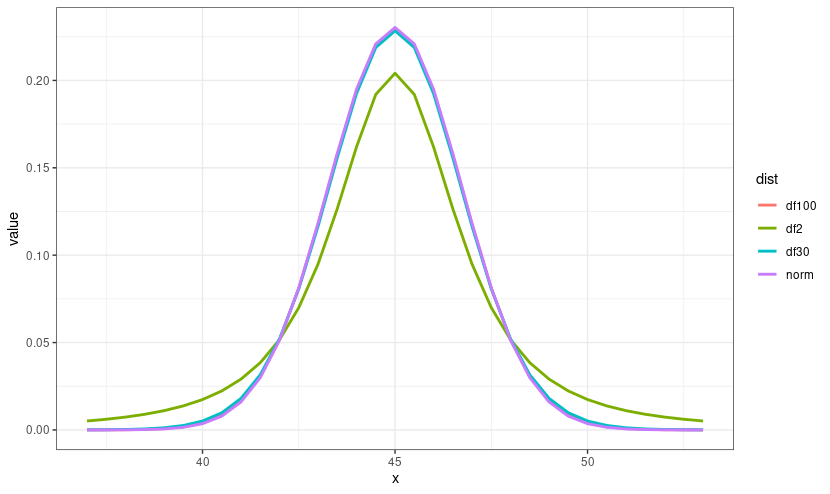
\includegraphics[scale=0.35]{pictures/densities.png}
        \caption{$\mu = 45$, $\sigma^{2}= 3$.}
    \end{figure}
\end{frame}

\begin{frame}[fragile]
    \frametitle{Robustness of the intial parameters}
    \framesubtitle{Testing random intial parameters}
\begin{minted}{R}
test_robustness <- function(mu, sigma, nu, n) {
    result <- vector("list", n)
    initial_par <- numeric(2 * n)
    dim(initial_par) <- c(n, 2)
    X <- extraDistr::rlst(2000, df = nu, mu = mu, sigma = sqrt(sigma))
    for(i in 1:n) {
        mu_r <- rcauchy(1, location = mu, scale = 100)
        sigma_r <- extraDistr::rpareto(1, a = 0.15, b = sigma)
        initial_par[i, 1] <- mu_r
        initial_par[i, 2] <- sigma_r
        result[[i]] <- EM(c(mu_r, sigma_r), X, nu)
    }
    list(results = result, initial_par = initial_par)
}
\end{minted}
\end{frame}

\begin{frame}
    \frametitle{Robustness of the intial parameters}
    \framesubtitle{Testing random intial parameters}
    Testing initial parameters with $\mu = 0$, $\sigma^{2} = 3$.
    \begin{figure}
        \centering
        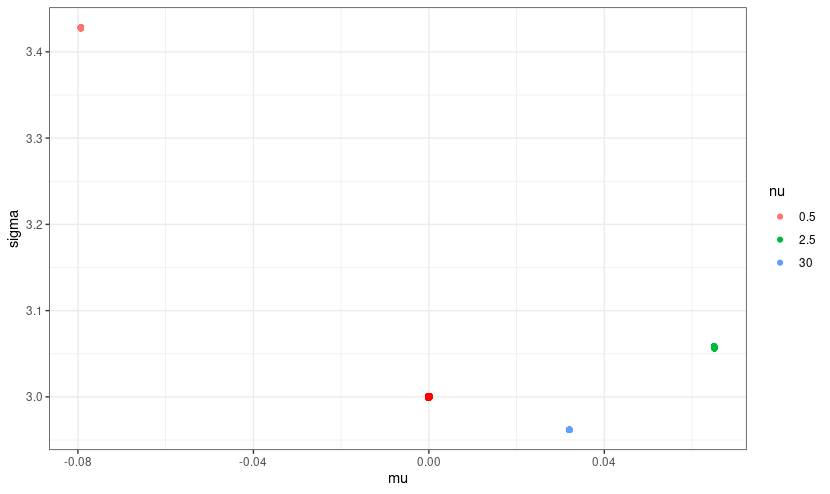
\includegraphics[scale=0.4]{pictures/ConvergentRobustness.png}
    \end{figure}
\end{frame}

\begin{frame}
    \frametitle{Robustness of the intial parameters}
    \framesubtitle{Testing random intial parameters}
    Testing initial parameters with $\mu = 0$, $\sigma^{2} = 3$.
    \begin{figure}
        \centering
        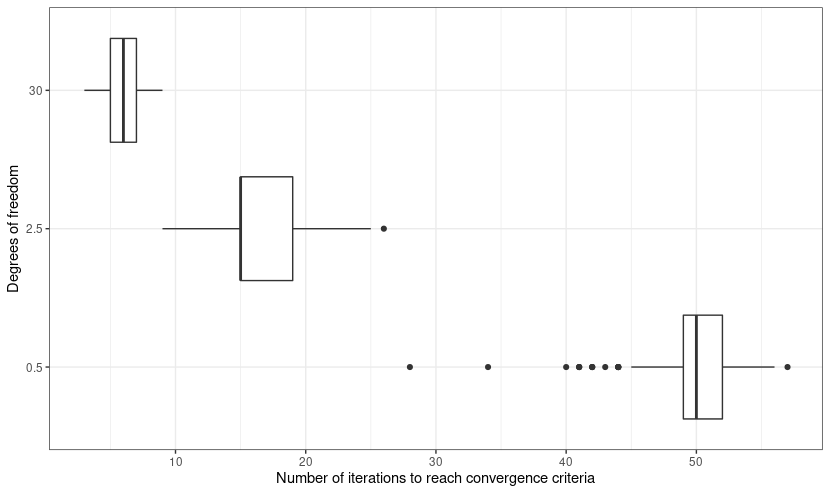
\includegraphics[scale=0.4]{pictures/IterationsToConvergenceRobustness.png}
    \end{figure}
\end{frame}

\begin{frame}[fragile]
    \frametitle{Automatic inital parameters}
    \framesubtitle{Median and inter quantile range}
    Sample mean and sample variance are unstable for $\nu < 2$. Suggestion: use inital $\theta_{0}=(\text{median}(X), \text{IQR}(X))$.
\begin{minted}{R}
EM <- function(par = NULL, x, nu, maxit = 500, min.eps = 1e-7) {
    E <- E_step(x, nu)
    M <- M_step(x, nu) 
    if(is.null(par)) {
        par <- c(median(x), IQR(x))
    }
    .
    .
    .
\end{minted}
\begin{minted}{R}
test_robustness2 <- function(mu, sigma, nu, n) {
    result <- vector("list", n)
    
    for(i in 1:n) {
        X <- extraDistr::rlst(2000, df = nu, mu = mu, sigma = sqrt(sigma))
        result[[i]] <- EM(x = X, nu = nu)
    }
    result
}
\end{minted}
\end{frame}
\begin{frame}
    \frametitle{Automatic inital parameters}
    \framesubtitle{Testing of automatic parameters} 
    Using $\mu = 0$ and $\sigma = 3$.
    \begin{figure}
        \centering
        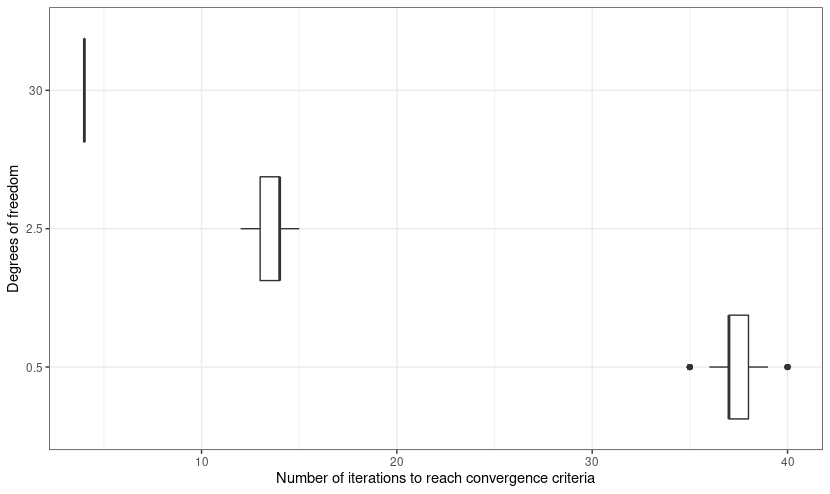
\includegraphics[scale=0.4]{pictures/automatic.png}
    \end{figure}
\end{frame}

\begin{frame}
    \frametitle{Newton-Methods}
    \framesubtitle{MLE directly from the marginal log-likelihood}
    Instead of using the EM algorithm to maximize the marginal likelihood one could maximize the likelihood directly:
    \begin{equation}
        \ell(\theta)\simeq-\frac{n}{2}\log\sigma^{2}-
        \frac{\nu+1}{2}\sum_{i=1}^{n}\log\left(1+\frac{(X_{i}-\mu)^{2}}{\nu\sigma^{2}}\right).
    \end{equation}
    We have the gradient
    \begin{align*}
        &\frac{\partial}{\partial\mu}\ell(\theta)= \frac{\nu + 1}{\nu\sigma^2}\sum_{i=1}^{n}\frac{X_{i} - \mu}{1 + \frac{(X_{i}-\mu)^2}{\nu\sigma^2}} \\
        &\frac{\partial}{\partial\sigma^{2}}\ell(\theta) = -\frac{n}{2\sigma^2} +
        \frac{\nu + 1}{2\nu(\sigma^2)^2}\sum_{i=1}^{n}\frac{(X_{i}-\mu)^2}{1 + \frac{(X_{i}-\mu)^2}{\nu\sigma^2}}    
    \end{align*}
\end{frame}

\begin{frame}[fragile]
    \frametitle{First Order Methods}
    \framesubtitle{Direct optimization of the marignal likelihood}
    Implemented minimizing the negative average log likelihood
    \begin{equation}
        -\frac{1}{n}\sum_{i=1}^{n}\ell_{i}(\theta).
    \end{equation}
\begin{minted}{R}
logl <- function(x, nu) {
    n <- length(x)
    force(nu)
    
    function(par) {
        mu <- par[1]
        sigma <- par[2]
        
        K <- sum(log(1 + (x - mu)^2 / (nu * sigma)))
        
        log(sigma) / 2 + (nu + 1) * K / (2 * n)
    }
}
\end{minted}
\end{frame}
\begin{frame}[fragile]
    \frametitle{First Order Methods}
    \framesubtitle{Direct optimization of the marignal likelihood}
\begin{minted}{R}
gradl <- function(x, nu) {
    n <- length(x)
    force(nu)
    
    function(par) {
        mu <- par[1]
        sigma <- par[2]
        
        C1 <- (x - mu) / (1 + (x - mu)^2 / (nu * sigma))
        
        K_mu <- sum(C1)
        K_sigma <- sum(C1 * (x - mu))
        
        grad_mu <- -(nu + 1) * K_mu / (n * nu * sigma)
        grad_sigma <- 1 / (2 * sigma) - (nu + 1) * K_sigma / (2 * n * nu * sigma^2)
        
        c(grad_mu, grad_sigma)
    }
}
\end{minted}
\end{frame}
\begin{frame}[fragile]
    \frametitle{First Order Methods}
    \framesubtitle{Implementation of Gradient Descent with backtracking}
\begin{minted}{R}
GD <- function(par, H, gr, d = 0.8, c = 0.1, gamma0 = 1, epsilon = 1e-7, maxiter = 500, cb = NULL
) {
    for(i in 1:maxiter) {
    value <- H(par)
    grad <- gr(par)
    h_prime <- sum(grad^2)
    gamma <- gamma0
    par1 <- par - gamma * grad
    if(!is.null(cb)) cb()
    while(min(H(par1), Inf, na.rm = TRUE) > value - c * gamma * h_prime) {
        gamma <- d * gamma
        par1 <- par - gamma * grad
    }
    if(norm(par - par1, "2") < epsilon * (norm(par, "2") + epsilon)) break
    par <- par1
    }
    if(i == maxiter) warning("Maximal number, ", maxiter, ", of iterations reached")
    par1
}    
\end{minted}
\end{frame}
\begin{frame}[fragile]
    \frametitle{First Order Methods}
    \framesubtitle{Implementation of the Conjugate Gradient Descent algorithm}
\begin{minted}[fontsize=\fontsize{6pt}{6pt}]{R}
CG <- function(par, H, gr, d = 0.8, c = 0.1, gamma0 = 1, epsilon = 1e-7, maxiter = 500, cb = NULL) {
    p <- length(par)
    m <- 1
    rho0 <- numeric(p)
    for(i in 1:maxiter) {
    value <- H(par)
    grad <- gr(par)
    grad_norm_sq <- sum(grad^2)
    if(!is.null(cb)) cb()
    gamma <- gamma0
    rho <- - grad + grad_norm_sq * rho0
    h_prime <- drop(t(grad) %*% rho)
    if(m > p || h_prime >= 0) {
        rho <- - grad
        h_prime <- - grad_norm_sq 
        m <- 1
    }
    par1 <- par + gamma * rho
    while(min(H(par1), Inf, na.rm = TRUE) > value + c * gamma * h_prime) {
        gamma <- d * gamma
        par1 <- par + gamma * rho
    }
    rho0 <- rho / grad_norm_sq
    if(norm(par - par1, "2") < epsilon * (norm(par, "2") + epsilon)) break
    par <- par1
    m <- m + 1
    }
    if(i == maxiter) warning("Maximal number, ", maxiter, ", of iterations reached")
    par1
}
\end{minted}
\end{frame}

\begin{frame}[fragile]
    \frametitle{Second Order Methods}
    \framesubtitle{Implementation of the Hessian}

\begin{minted}[fontsize=\fontsize{8pt}{8pt}]{R}
hessl <- function(x, nu) {
    n <- length(x)
    force(nu)
    function(par){
        mu <- par[1]
        sigma <- par[2]
        
        C0 <- 1 / (1 + (x - mu)^2 / (nu * sigma))
        C1 <- C0 * (x - mu)
        C2 <- C1 * (x - mu)
        
        hess_mu <- (nu + 1) * sum(C0) / (n * nu * sigma) + 
            2 * (nu + 1) * sum(C1^2) / (n * (nu * sigma)^2)
        
        hess_sigma <- -1 / (2 * sigma^2) + 
            (nu + 1) * sum(C2) / (n * nu * sigma^3) -
            (nu + 1) * sum(C2^2) / (2 * n * nu^2 * sigma^4)
    
        hess_mu_sigma <- (nu + 1) * sum(C1) / (n * nu * sigma^2) -
            (nu + 1) * sum(C1^2 * (x - mu)) / (n * nu * sigma^3)
        
        hess <- c(hess_mu, hess_mu_sigma, hess_mu_sigma, hess_sigma)
        dim(hess) <- c(2, 2)
        hess
    }
}
\end{minted}
\end{frame}

\begin{frame}[fragile]
    \frametitle{Second Order Methods}
    \framesubtitle{Implementation of Newton algorithm with backtracking and Wolff line search}
\begin{minted}[fontsize=\fontsize{7pt}{7pt}]{R}
Newton <- function(par, H, gr, hess, d = 0.8, c = 0.2, gamma0 = 1, epsilon = 1e-7, maxiter = 500, cb = NULL) {
    for(i in 1:maxiter) {
        value <- H(par)
        grad <- gr(par)
        if(!is.null(cb)) cb()
        Hessian <- hess(par) 
        rho <- - drop(solve(Hessian, grad)) 
        gamma <- gamma0
        par1 <- par + gamma * rho
        h_prime <- t(grad) %*% rho 
        while(min(H(par1), Inf, na.rm = TRUE) > value +  c * gamma * h_prime) { 
            gamma <- d * gamma 
            par1 <- par + gamma * rho
        }
        if(norm(par - par1, "2") < epsilon * (norm(par, "2") + epsilon)) break
        par <- par1 
    }
    if(i == maxiter) warning("Maximal number, ", maxiter, ", of iterations reached")
    par1
}      
\end{minted}
\end{frame}

\begin{frame}
    \frametitle{Comparisons of algorithms}
    \framesubtitle{Comparison of convergence}
    The convergence criteria is identical for both algorithms. When either the algorithms reach $500$ iterations or $||\theta_{n+1} -\theta_{n}||<\varepsilon(||\theta_{n}||+\varepsilon)$ for $\varepsilon = 10^{-7}$.\\[12pt]
    $10.000$ samples of the t-distribution with parameters $\mu = 5$, $\sigma^{2}=2$ and $\nu = 3$. For the GD, CGD and Newton algorithms the paremters $\texttt{d} = 0.8$, $\texttt{c} = 0.2$ and $\texttt{gamma0} = 1$ were used. All algorithms reached convergence before 500 iterations.
    \begin{align*}
        &\hat\theta_{\text{GD}}=(5.013613671, 2.051342021) \quad \ell(\hat\theta_{\text{GD}})=1.12761474375058723\\
        &\hat\theta_{\text{CG}}=(5.013613671, 2.051342056) \quad \ell(\hat\theta_{\text{CG}})=1.12761474375060544\\
        &\hat\theta_{\text{NT}}=(5.013613344, 2.051333484) \quad \ell(\hat\theta_{\text{NT}})=1.12761474374844051\\
        &\hat\theta_{\text{EM}}=(5.013613675, 2.051333775) \quad \ell(\hat\theta_{\text{EM}})=1.12761474374842496
    \end{align*}
\end{frame}
\begin{frame}
    \frametitle{Comparisons of algorithms}
    \framesubtitle{Development of the $\mu$-estimate}
    \begin{figure}
        \centering
        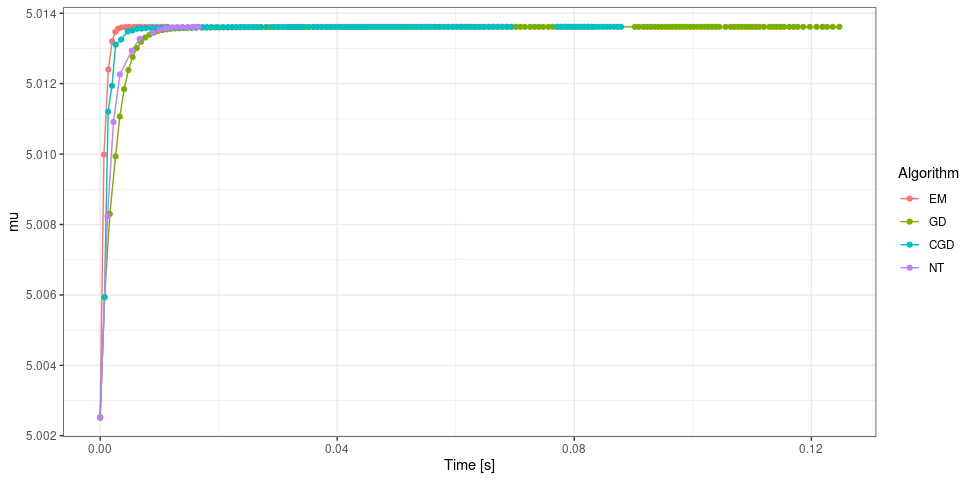
\includegraphics[scale = 0.4]{pictures/NewComp/AllMuNu3.png}
    \end{figure}
\end{frame}
\begin{frame}
    \frametitle{Comparisons of algorithms}
    \framesubtitle{Development of the $\sigma^{2}$-estimate}
    \begin{figure}
        \centering
        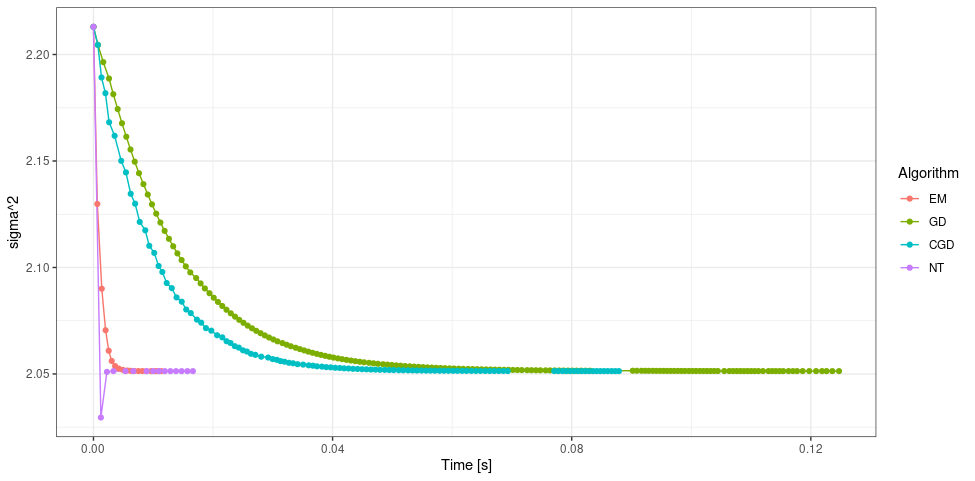
\includegraphics[scale = 0.4]{pictures/NewComp/AllSigmaNu3.png}
    \end{figure}
\end{frame}
\begin{frame}
    \frametitle{Comparisons of algorithms}
    \framesubtitle{Development of the distance between parameters}
    \begin{figure}
        \centering
        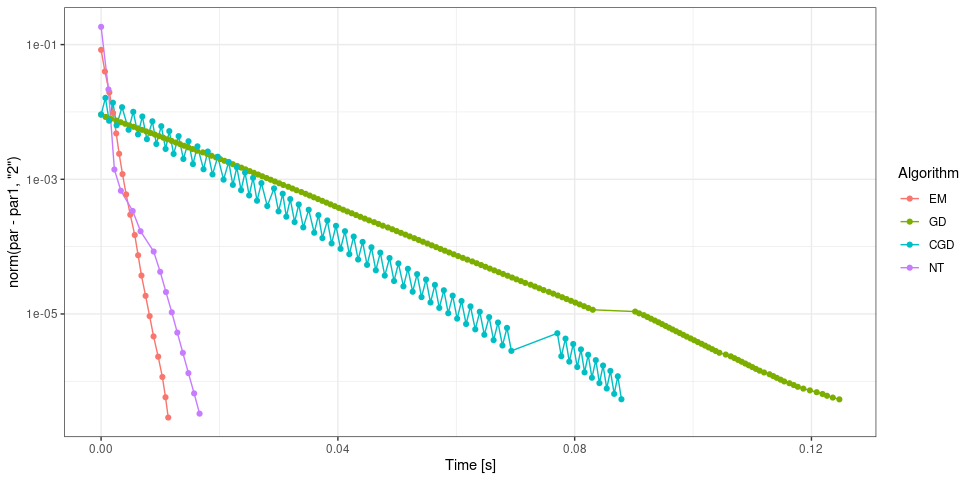
\includegraphics[scale = 0.4]{pictures/NewComp/AllNormNu3.png}
    \end{figure}
\end{frame}
\begin{frame}
    \frametitle{Comparisons of algorithms}
    \framesubtitle{Parameters matter}
    Choosing $\texttt{gamma0} = 6$ for the GD and CGD algorithms yields
    \begin{figure}
        \centering
        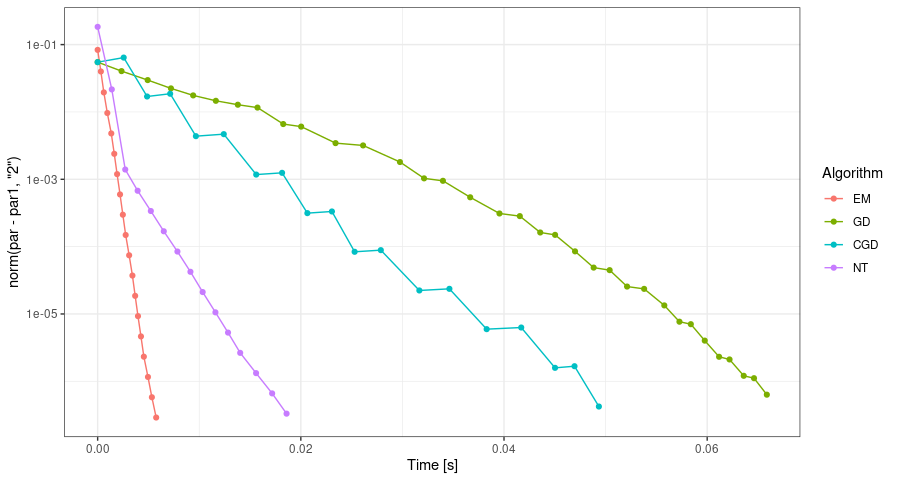
\includegraphics[scale = 0.4]{pictures/NewComp/ChangedParameters.png}
    \end{figure}
\end{frame}

\begin{frame}
    \frametitle{Comparison of algorithms}
    \framesubtitle{Convergence for small $\nu$}
    Repeating the same experiment with $\nu = 0.5$. The GD and CGD algorithms did not reach convergence before 500 iterations.
    \begin{align*}
        &\hat\theta_{\text{GD}}=(4.985824153, 2.107854186) \quad \ell(\hat\theta_{\text{GD}})=2.75212300025436729\\
        &\hat\theta_{\text{CG}}=(4.985815963, 2.103884595) \quad \ell(\hat\theta_{\text{CG}})=2.75212286766256398\\
        &\hat\theta_{\text{NT}}=(4.985814613, 2.103818326) \quad \ell(\hat\theta_{\text{NT}})=2.75212286762692315\\
        &\hat\theta_{\text{EM}}=(4.985815835, 2.103821265) \quad \ell(\hat\theta_{\text{EM}})=2.75212286762684455
    \end{align*}
\end{frame}

\begin{frame}
    \frametitle{Comparisons of algorithms}
    \framesubtitle{Development of the $\mu$-estimate}
    \begin{figure}
        \centering
        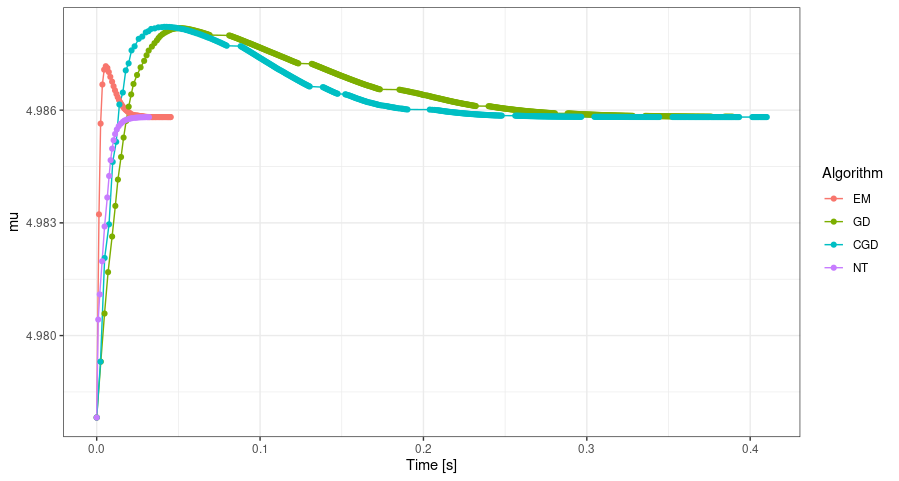
\includegraphics[scale = 0.4]{pictures/NewComp/AllMuNu0_5.png}
    \end{figure}
\end{frame}
\begin{frame}
    \frametitle{Comparisons of algorithms}
    \framesubtitle{Development of the $\sigma^{2}$-estimate}
    \begin{figure}
        \centering
        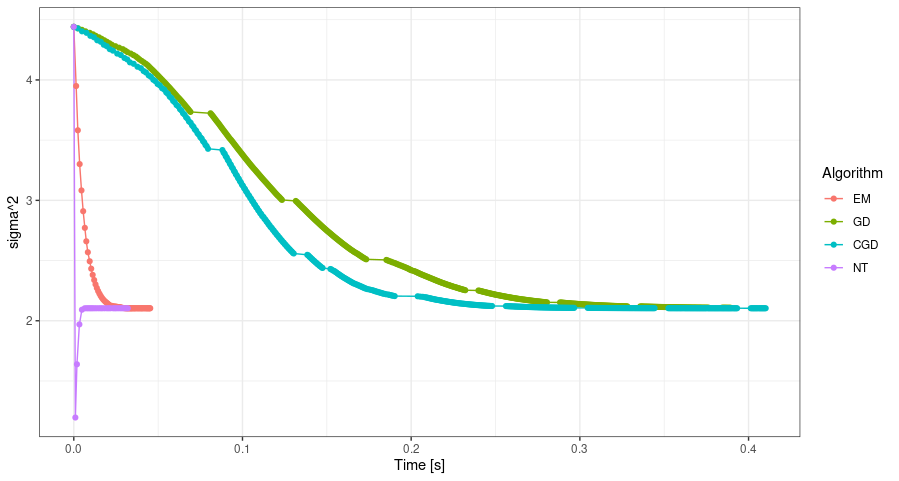
\includegraphics[scale = 0.4]{pictures/NewComp/AllSigmaNu0_5.png}
    \end{figure}
\end{frame}
\begin{frame}
    \frametitle{Comparisons of algorithms}
    \framesubtitle{Development of the distance between parameters}
    \begin{figure}
        \centering
        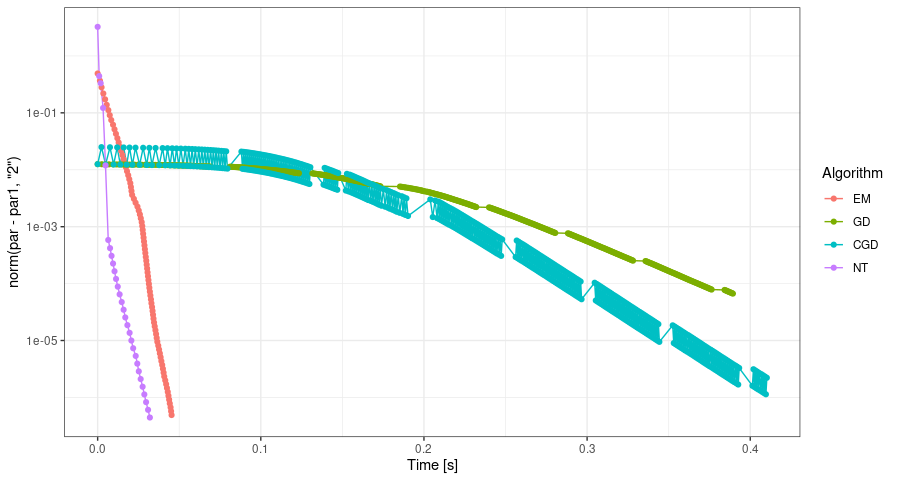
\includegraphics[scale = 0.4]{pictures/NewComp/AllNormNu0_5.png}
    \end{figure}
\end{frame}
\begin{frame}
    \frametitle{Comparisons of algorithms}
    \framesubtitle{Stability of algorithms}
    If $\nu = 0.2$ then the Newton algorithm no longer works. It gets stuck in backtracking. The initial guess $(\text{median}(X), \text{IQR}(X))$ is too far off --- in particular the guess of $\sigma^{2}$ is not very good.
    \begin{figure}
        \centering
        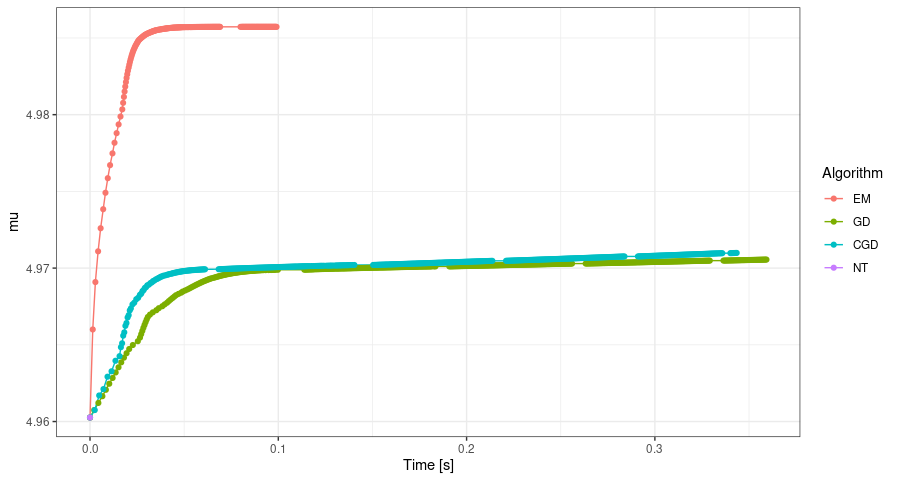
\includegraphics[scale = 0.4]{pictures/NewComp/AllMuNu0_2.png}
    \end{figure}
\end{frame}
\begin{frame}
    \frametitle{Comparisons of algorithms}
    \framesubtitle{Stability of algorithms}
    \begin{figure}
        \centering
        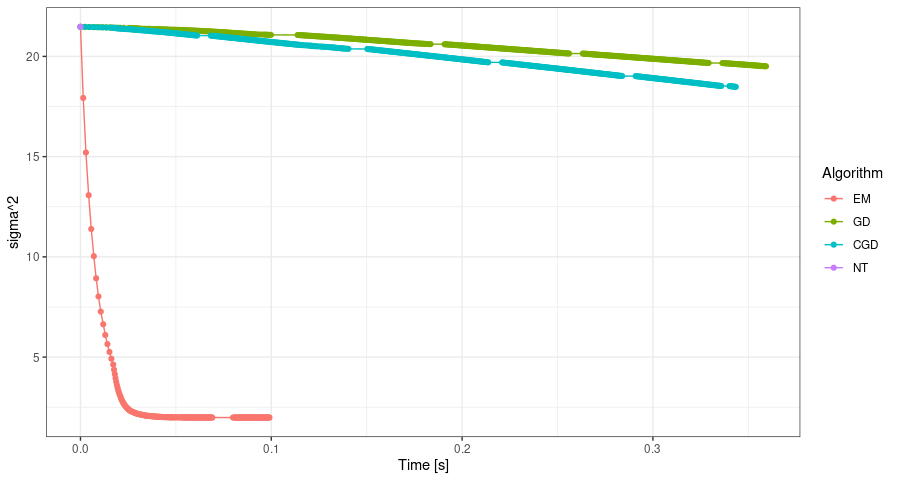
\includegraphics[scale = 0.4]{pictures/NewComp/AllSigmaNu0_2.png}
    \end{figure}
\end{frame}
\begin{frame}
    \frametitle{Comparisons of algorithms}
    \framesubtitle{Stability of algorithms}
    \begin{figure}
        \centering
        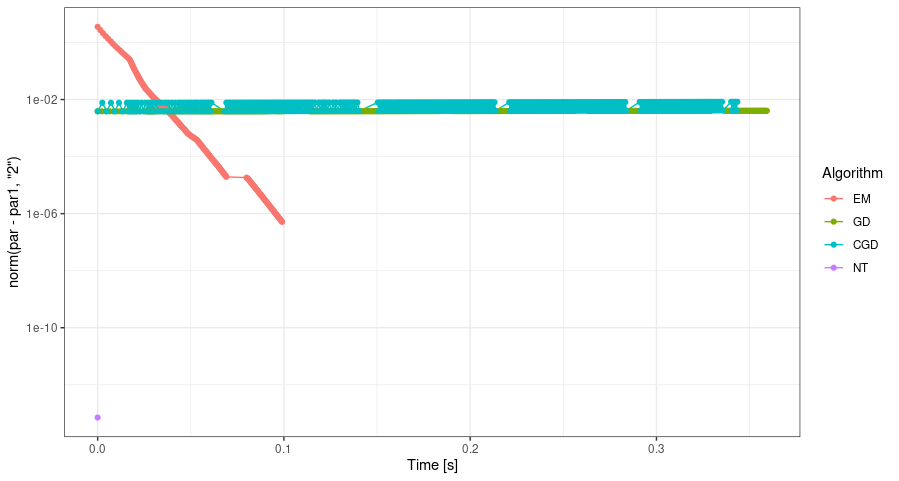
\includegraphics[scale = 0.4]{pictures/NewComp/AllNormNu0_2.png}
    \end{figure}
\end{frame}
\begin{frame}
    \frametitle{Profiling of the Newton algorithm}
    Using 10.000.000 samples with $\mu = 5$, $\sigma^{2} = 2$ and $\nu = 1.5$.
    \begin{figure}
        \centering
        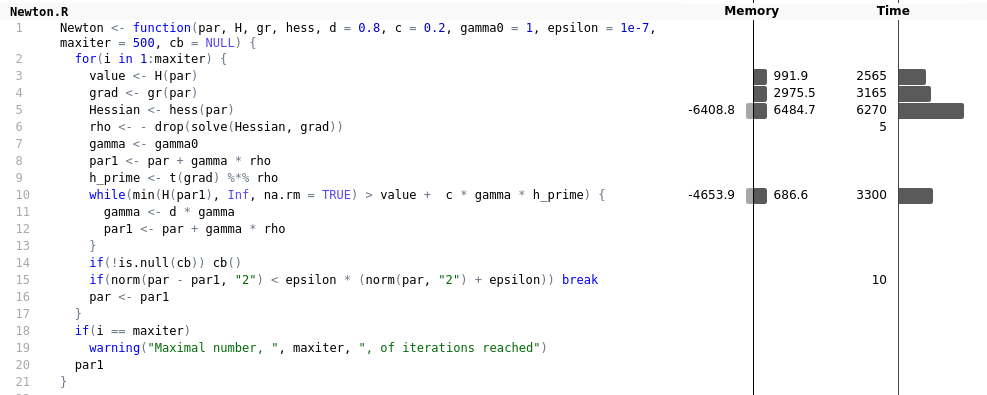
\includegraphics[scale = 0.4]{pictures/NewtonProfile.png}
    \end{figure}
\end{frame}
\begin{frame}
    \frametitle{Profiling of the EM algorithm}
    Using 10.000.000 samples with $\mu = 5$, $\sigma^{2} = 2$ and $\nu = 1.5$.
    \begin{figure}
        \centering
        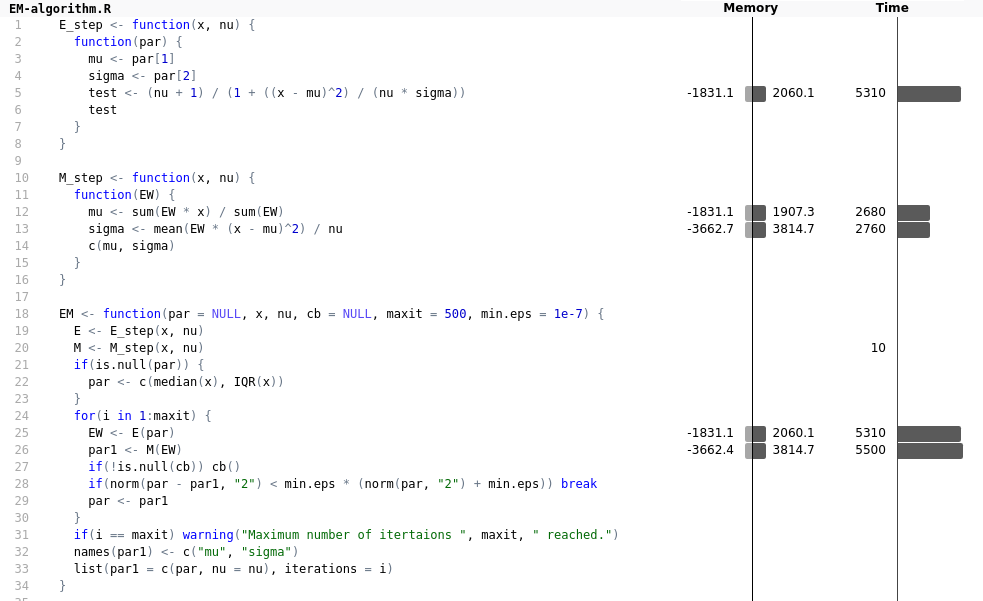
\includegraphics[scale = 0.32]{pictures/EMProfile.png}
    \end{figure}
\end{frame}
\begin{frame}
    \frametitle{Calculating the fisher information}
    \framesubtitle{Methods of calculation the fisher information}

\end{frame}
\end{document}
